\chapter{基于hp自适应伪谱法的再入轨迹设计与分析}

飞船再入环境严苛,整个再入段受热流、过载、动压等约束的影响。应急条件下,飞船为到达目标着陆场,再入轨迹存在不同的轨迹形式。本章研究飞船再入机动可达域的快速确定问题,利用伪谱方法完成不同再入轨迹形式下的可达域确定。通过容许不同的轨迹形式,扩展再入点的范围,为应急返回提供更大的窗口。

\section{再入返回轨迹设计问题建模}
\subsection{再入动力学方程}
在探月飞船再入返回轨迹设计问题中,采用三自由度运动模型,采用“瞬时平衡假设”,认为返回器始终以配平攻角飞行,且侧滑角为零。考虑地球自转,圆球假设下,忽略地球扁率和侧滑角等的影响,在半速度系下建立运动方程,以时间为自变量的飞船无动力再入动力学方程满足
\begin{equation}
	\left\{
	\begin{aligned}
		\frac{\dif r}{\dif t}=       & v \sin \theta                                                           \\
		\frac{\dif \lambda}{\dif t}= & \frac{v \cos \theta \sin \psi}
		{r \cos \phi}                                                                                          \\
		\frac{\dif \phi}{\dif t}=    & \frac{v \cos \theta \cos \psi}{r}                                       \\
		\frac{\dif v}{\dif t}=       & -D-g \sin \theta +\omega_e^2r\cos\phi \sin\theta \cos\phi-
		\omega_e^2r\cos\phi\cos\theta\sin\phi\cos\sigma                                                        \\
		\frac{\dif\theta}{\dif t} =  & \frac{L\cos\sigma}{v}+(\frac{v}{r}-
		\frac{g}{v})\cos\theta+2\omega_e\cos\phi\sin\sigma                                                     \\
		                             & {}+\frac{\omega_e^2r\cos\phi\cos\theta\cos\phi}{v}                      \\
		\frac{\dif\psi}{\dif t} =    & \frac{L\sin\sigma}{v\cos\theta}+\frac{v\sin \psi\cos \theta\tan\phi}{r}
		-2\omega_e(\cos\phi\tan\theta\cos\sigma-\sin\phi)                                                      \\
		                             & {}+\frac{\omega_e^2r}{\cos\theta}sin\phi\cos\phi\sin\sigma
	\end{aligned}
	\right.
\end{equation}
其中,$r$为地心距,$\lambda$和$\phi$为经纬度,$v$为相对地球速度,$\theta$为当地速度倾角,表征速度与当地水平的夹角,以及$\psi$为速度方位角,表征速度在当地水平面内的投影与当地正北方向的夹角,顺时针为正;$\sigma$为控制量倾侧角,反映了升力对铅锤面的倾斜;$ \omega_e $为地球自转角速度,$L$,$D$为再入过程中的升力阻力加速度,满足
\begin{align}
	L & =\frac{C_L\rho v^2S}{2m} \\
	D & =\frac{C_D\rho v^2S}{2m}
\end{align}
其中:$ C_L $和$ C_D $为气动升力系数和气动阻力系数,$ \rho $为大气密度,$ m $为飞行器质量,$ S $为飞船的参考面积。

大气密度$ \rho $可采用指数模型、多阶段拟合公式和美国US1976标准大气模型等,考虑到精度和计算速度的要求,最终采用多阶段的拟合公式,更多可参考\upcite{贾沛然-1993-远程火箭弹道学}。
\begin{equation}
	\rho=\rho_0 e^{-\beta h}
\end{equation}

\subsection{约束分析}
因探月返回器高速再入的特点,过载和热流等约束十分苛刻。为了保证再入过程的安全,根据约束的性质划分为两类:过程约束和终端约束。
\subsubsection{过程约束}
\begin{enumerate}
	\item 热流约束\par
	      高超声速气动加热对热防护系统(TPS)的影响,为避免飞行器被烧毁,因此需对飞行器再入过程中的热流密度进行限制。
	      通常采用驻点热流密度作为约束指标,计算公式如下:
	      \begin{equation}
		      \dot{Q} = k_s\left(\frac{\rho}{\rho_{0}}\right)^{0.5}\left(\frac{v}{V_{c}}\right)^{m}
	      \end{equation}
	      其中,$ k_s $为热流相关常数,$ V_c=7.9\mathrm{km/s} $为参考的第一宇宙速度,$ m $可取3或3.15,本文中取3.15
	\item 过载约束\par
	      考虑到内部结构、材料的限制,需要对过载进行限制,要求瞬时过载小于最大允许过载,即
	      \begin{equation}
		      n=\sqrt{{{L}^{2}}+{{D}^{2}}}\le {{n}_{\max }}
	      \end{equation}
	      其中,$ n_{\max} $为最大允许过载值。
	\item 动压约束\par
	      动压对控制系统的影响和侧向稳定性的要求,
	      \begin{equation}
		      q=\frac{1}{2} \rho V^{2} \leq q_{\max }
	      \end{equation}
	\item 跃起高度约束\par
	      此外,为防止跳出高度过高导致任务失败,路径约束还应包括一个高度约束。这里设定最大高度不超过300km,
	      \begin{equation}
		      h<h_{\max}
	      \end{equation}
	\item 控制量约束\par
	      控制量倾侧角受限于执行机构,飞船的控制能力有限,实际倾侧角机动不可能瞬时完成,需要对倾侧角和倾侧角变化速率进行限幅,即
	      \begin{equation}
		      \left\{
		      \begin{aligned}
			      \abs{\sigma}       & \leq \sigma_{\max}       \\
			      \abs{\dot{\sigma}} & \leq \dot{\sigma}_{\max} \\
		      \end{aligned} \right.
	      \end{equation}
\end{enumerate}

\subsubsection{终端约束}
对于再入问题中的终端约束,包含起始点和终点的状态约束。起始点处的状态在分析中通常为给定值,在初始时刻$ t_0 $状态满足
\begin{equation}
	\left\{ \begin{aligned}
		h(t_0)=h_0,\lambda(t_0)=\lambda_0,\phi(t_0)=\phi_0 \\
		v(t_0)=v_0,\theta(t_0)=\theta_0,\psi(t_0)=\psi_0
	\end{aligned} \right.
\end{equation}

终点处根据研究问题可分为固定终点和自由终点两种情况,数学上表达为:
\begin{enumerate}
	\item 固定终点的约束条件\par
	      终点处位置固定,但速度和速度倾角存在范围约束,即:
	      \begin{equation}
		      \left\{ \begin{aligned}
			      h(t_f) & =h_{f}, \lambda(t_f)=\lambda_{f}, \phi(t_f)=\phi_{f}       \\
			      v      & \geq v_{f}, \theta_{\min } \leq \theta \leq \theta_{\max }
		      \end{aligned}\right.
	      \end{equation}
	\item 自由终点的约束条件\par
	      对于求解可达域等问题时,终点不固定,通常约束设置为:
	      \begin{equation}
		      h(t_f)=h_{f}, v \geq v_{f}, \theta_{\min } \leq \theta \leq \theta_{\max }
	      \end{equation}
\end{enumerate}

\section{hp自适应伪谱法的求解策略}
hp自适应伪谱法是伪谱方法的一种,求解再入问题在计算速度有较大优势。hp自适应伪谱法主要包含两部分内容:伪谱化离散和hp自适应网格细化。
\subsection{LGR离散化方法}
%在绪论中介绍轨迹优化问题描述
首先将在连续时间$ [t_0,t_f] $上的问题划分为$ K $个子区间,记第$ k $个子区间为$ [t_{k-1},t_k] $,有$ t_0<t_1<t_2<\ldots<t_k $。对于
第k个子区间,首先需要将时域$ t\in[t_{k-1},t_k] $,转换到$ \tau \in [-1,1] $,即:
\begin{equation}
	\tau = \frac{2 t-\left(t_{k-1}+t_{k}\right)}{t_{k}-t_{k-1}}
	\label{eq:time Trans}
\end{equation}

经过区间划分后,$ [t_0,t_f] $时间内的连续优化问题可以表述为:
\begin{enumerate}
	\item 动力学方程
	      \begin{equation}
		      \frac{\dif \boldsymbol{x}^{(k)}(\tau)}{\dif \tau}=\frac{t_{k}-t_{k-1}}{2} f\left(\boldsymbol{x}^{(k)}(\tau), \boldsymbol{u}^{(k)}(\tau)\right), \quad(k=1, \cdots, K)
	      \end{equation}
	\item 目标函数
	      \begin{equation}
		      J=\Phi\left(\boldsymbol{x}^{(1)}(-1), t_{0}, \boldsymbol{x}^{(K)}(+1), t_{K}\right)+\sum_{k=1}^{K} \frac{t_{k}-t_{k-1}}{2} \int_{t_{0}}^{t_{f}} g\left(\boldsymbol{x}^{(k)}(\tau), \boldsymbol{u}^{(k)}(\tau)\right) d \tau
	      \end{equation}
	\item 路径约束
	      \begin{equation}
		      \frac{t_{k}-t_{k-1}}{2} \boldsymbol{C}\left(\boldsymbol{x}^{(k)}(\tau), \boldsymbol{u}^{(k)}(\tau)\right) \leq 0 \quad(k=1, \cdots, K)
	      \end{equation}
	\item 边界条件
	      \begin{equation}
		      \phi\left(\boldsymbol{x}^{(1)}(-1), t_{0}, \boldsymbol{x}^{(K)}(+1), t_{K}\right)=0
	      \end{equation}
\end{enumerate}

引入区间划分后,附加产生额外的内点约束:
\begin{equation}
	\phi\left(\boldsymbol{x}^{(1)}(-1), t_{0}, \boldsymbol{x}^{(K)}(+1), t_{K}\right)=0
\end{equation}

进一步,需要对问题进行离散化求解。Radau伪谱法的配点为Legendre-Gauss-Radau(LGR)点,LGR点相对于原点是不对称的,并且不是唯一的,
可以使用初始点或终点来定义它们。一般的LGR点配置在 $ [t_{k-1},t_k) $上(包含起点),将其归一化后,即端点$ \tau_{N_k+1}^{(k)}=+1 $为非配点。区间内的离散点为$ -1=\tau_1<\tau_2<\cdots<\tau_{N_k}<\tau_{N_k+1} $,此处省略上标$ k $。
对于任意一个子区间$  [t_{k-1},t_k] $,取$ N_k $个LGR点,取插值点为$ N_k $个LGR点与终端点$ \tau_{N_k+1}^{(k)}=+1 $,状态量的近似可以表示为:
\begin{equation}
	\boldsymbol{x}^{(k)}(\tau) \approx \boldsymbol{X}^{(k)}(\tau)=\sum_{j=1}^{N_{k}+1} \boldsymbol{X}_{j}^{(k)} L_{j}^{(k)}(\tau)
	\label{eq:state}
\end{equation}
其中,简记$ \boldsymbol{X}_{j}^{(k)}=\boldsymbol{X}^{(k)}\left(\tau_{j}^{(k)}\right)$,$ \quad L_{j}^{(k)}(\tau) $为Lagrange插值
基函数:
\begin{equation}
	L_{j}^{(k)}(\tau)=\prod_{i=1, i \neq j}^{N_{k}+1} \frac{\tau-\tau_{i}^{(k)}}{\tau_{j}^{(k)}-\tau_{i}^{(k)}}
\end{equation}

获得状态量的近似后,进一步对于动力学方程的状态导数可以近似为:
\begin{equation}
	\frac{\dif \boldsymbol{x}^{(k)}(\tau)}{\dif \tau} \approx \frac{\dif \boldsymbol{X}^{(k)}(\tau)}{\dif \tau}=\sum_{j=1}^{N_{k}+1} \boldsymbol{X}_{j}^{(k)} \dot{L}_{j}^{(k)}(\tau)
\end{equation}

状态量的近似通过在$ N_k+1 $个插值点处的Lagrange插值多项式近似,对于控制量通过在$ N_k $个配点处插值获得,有:
\begin{equation}
	\boldsymbol{u}^{(k)}(\tau) \approx \boldsymbol{U}^{(k)}(\tau)=\sum_{i=1}^{N_{k}} \boldsymbol{U}_{i}^{(k)}\widetilde{L}_{i}^{(k)}(\tau)
	\label{eq:control}
\end{equation}
其中$ \widetilde{L}_{i}^{(k)}(\tau) $与$ L_{j}^{(k)}(\tau) $具有类似的形式,此处不再列出。

经过\eqref{eq:state}-\eqref{eq:control}的处理,连续时间上的原最优控制问题可转化为其离散形式:
\begin{enumerate}
	\item 动力学方程\par
	      在配点处,原动力学微分方程约束转换为代数约束形式,表达为:
	      \begin{equation}
		      \sum_{j=1}^{N_{k}+1} \boldsymbol{X}_{j}^{(k)} D_{i j}^{(k)}-\frac{t_{k}-t_{k-1}}{2} \boldsymbol{f}_{i}^{(k)}=0, \quad\left(i=1, \cdots, N_{k}, k=1, \cdots, K\right)
	      \end{equation}
	      其中,$\boldsymbol{f}_{i}^{(k)}=\boldsymbol{f}\left(\boldsymbol{X}_{i}^{(k)}, \boldsymbol{U}_{i}^{(k)}\right)$,简记$ \boldsymbol{U}_{i}^{(k)}=\boldsymbol{U}^{(k)}\left(\tau_{i}^{(k)}\right)$,式中:
	      \begin{equation}
		      D_{i j}^{(k)}=\dot{L}_{j}^{(k)}\left(\tau_{i}^{(k)}\right) \quad\left(i=1, \cdots, N_{k}, j=1, \cdots, N_{k}+1\right)
	      \end{equation}
	      $ \left\{D_{i j}^{(k)}\right\} $为区间$ k $内大小$ N_k\times (N_k+1) $的微分矩阵,通常可以利用差分近似。
	\item 目标函数\par
	      目标函数转化为
	      \begin{equation}
		      J=\Phi\left(\boldsymbol{X}^{(1)}(-1), t_{0}, \boldsymbol{X}_{N_{K}+1}^{(K)}, t_{K}\right)+\sum_{k=1}^{K} \sum_{j=1}^{N_{K}} \frac{t_{k}-t_{k-1}}{2} w_{j}^{(k)} g_{j}^{(k)}
	      \end{equation}
	      其中,$w_{j}^{(k)}=\int_{-1}^{1} L_{j}^{(k)}(\tau) d \tau$为第k个子区间上的Legendre-Gauss权重,$g_{j}^{(k)}=g\left(\boldsymbol{X}_{j}^{(k)}, \boldsymbol{U}_{j}^{(k)}\right)$。
	\item 路径约束\par
	      \begin{equation}
		      \frac{t_{k}-t_{k-1}}{2} \boldsymbol{C}^{(k)}\left(\boldsymbol{X}_{i}^{(k)}, \boldsymbol{U}_{i}^{(k)}\right) \leq 0 \quad\left(i=1, \cdots, N_{k}, k=1, \cdots, K\right)
	      \end{equation}
	\item 边界条件\par
	      \begin{equation}\phi\left(\boldsymbol{X}^{(1)}(-1), t_{0}, \boldsymbol{X}_{N_{K}+1}^{(K)}, t_{K}\right)=0\end{equation}
	      同时离散化引入的附加内点约束变为:
	      \begin{equation}
		      \boldsymbol{X}_{N_{k}+1}^{(k)}=\boldsymbol{X}_{1}^{(k+1)}, \quad(k=1, \ldots, K-1)
	      \end{equation}
\end{enumerate}

文献【19】从近似精度和计算效率等方面对上述三种伪谱法进行了比较。 Radau伪谱法和Gauss伪谱法在状态变量、控制变量和共轭变量的近似精度上均优于 Legendre伪谱法,同时, Gauss伪谱法对共轭变量边界值的估计精度高于Radau伪谱法,且在处理含初始和终端约束的问题上具有优势。在计算效率方面,求解相同规模问题时三种方法耗时差别不大。

\subsection{hp自适应网格细化方法}
最早hp方法发展于求解偏微分方程中的有限元方法,进一步被引入到求解最优控制问题,解决不连续点上收敛速度慢的问题。hp方法是为提高求解精度和收敛速度的一种p方法和h方法的混合算法。p方法是保持通过提高插值多项式的阶次进行求解,全局的伪谱方法就是典型的p方法;h方法通过划分区间,固定区间内插值多项式的阶次,通过细化区间求解问题。hp方法能够综合p方法在光滑解条件下的指数收敛速度优势并且只在不连续的区域或者解发生突变处细化区间。研究\upcite{Darby-2011-Directtrajectoryoptimization,Darby-2011-hpadaptivepseudospectral}也表明hp方法相比于p方法和h方法,能够有效降低近似的维度。

hp方法的基本思想是:从初始网格出发,对每段的近似误差进行估计,通过增大插值多项式的阶次和对当前区间进行划分的方法对当前网格进行细化,重复直至精度满足要求。

\subsubsection{误差评估}
为衡量在区间$ [t_{k-1},t_k] $内动力学方程约束的满足情况,首先定义区间内的一系列评估误差的检验点,取为相邻配点的中点,有:
\begin{equation}
	\bar{t}_{i}=\frac{t_{i}+t_{i+1}}{2} \quad\left(i=1, \ldots, N_{k}-1\right)
\end{equation}

在这些检验点上,通过\eqref{eq:state}和\eqref{eq:control}获得这些点处的状态量$ \overline{\boldsymbol{X}} $和控制量$ \overline{\boldsymbol{U}} $的估计值,分别为$ (N_k-1)\times n $和$ (N_k-1)\times m $的矩阵,这里$ n $和$ m $分别为状态量和控制量的个数。
\begin{equation}
	\overline{\boldsymbol{X}}=\left[\begin{array}{c}
			\boldsymbol{X}\left(\bar{t}_{1}\right) \\
			\vdots                                 \\
			\boldsymbol{X}\left(\bar{t}_{N_{k}-1}\right)
		\end{array}\right], \quad \overline{\boldsymbol{U}}=\left[\begin{array}{c}
			\boldsymbol{u}\left(\bar{t}_{1}\right) \\
			\vdots                                 \\
			\boldsymbol{u}\left(\bar{t}_{N_{k}-1}\right)
		\end{array}\right]
\end{equation}

进一步,通过式\eqref{eq:time Trans}对时间进行时域变换,得到$ \tau=\left(\bar{\tau}_{1}, \ldots, \bar{\tau}_{N_{k}-1}\right) \in[-1,1] $。计算动力学约束的误差$ \boldsymbol{R} $为
\begin{equation}
	\boldsymbol{R}=\left|\bar{\boldsymbol{ D }} \bar{\boldsymbol{X}}-\frac{t_{k}-t_{k-1}}{2} \boldsymbol{F}\left(\overline{\boldsymbol{X}}, \overline{\boldsymbol{U}}, \tau ; \boldsymbol{p}, t_{k-1}, t_{k}\right)\right| \in \mathbb{R}^{\left(N_{k}-1\right) \times n}
	\label{eq:residual func}
\end{equation}
$ \boldsymbol{R} $为$ (N_k-1)\times n  $的矩阵,矩阵中的每列元素都代表了对应状态在配点间的违反程度。

% where denotes the absolute value of each element of the matrix R. The elements of the matrix R will be referred to as the midpoint residuals of the dynamics at the midpoints of the collocation points and the matrix R itself will be referred to as the midpoint residual matrix. Each column of the matrix r provides a measure of the amount by which the state violates the collocation equations at the midpoints between two collocation points in segment s

记矩阵$ \boldsymbol{R} $中最大元素所在列为$ \boldsymbol{r} $,$ \boldsymbol{r} $可以表示为
\begin{equation}
	\boldsymbol{r}=\left[\begin{array}{c}
			r\left(\bar{t}_{1}\right) \\
			\vdots                    \\
			r\left(\bar{t}_{N_{k}-1}\right)
		\end{array}\right]
\end{equation}

由于$ \boldsymbol{r} $中包含最大偏差处的信息,可以作为进一步划分区间或者增加插值多项式阶次的依据。

进一步,记$ \bar{r}$为向量,$ \boldsymbol{r} $的算术平均值,即:
\begin{equation}
	\bar{r}=\frac{\sum_{i=1}^{N_{k}-1} r\left(\bar{t}_{i}\right)}{N_{k}-1}
\end{equation}
定义
\begin{equation}
	\boldsymbol{\beta}=\left[\begin{array}{c}
			\beta\left(\bar{t}_{1}\right) \\
			\vdots                        \\
			\beta\left(\bar{t}_{N_{s}-1}\right)
		\end{array}\right]=\left[\begin{array}{c}
			r\left(\bar{t}_{1}\right) / \bar{r} \\
			\vdots                              \\
			r\left(\bar{t}_{N_{s}-1}\right) / \bar{r}
		\end{array}\right]
\end{equation}
$ \bm{\beta} $为尺度变换后的在检验点处的偏差向量,代替$ \boldsymbol{r} $作为后续细化策略的依据。
\subsubsection{细化策略}
对于向量$ \bm{\beta} $,存在两种情况,分别对应细化区间和增加插值多项式阶次两种策略:
\begin{enumerate}
	\item 当$ \bm{\beta} $中的元素都很小时,认为在区间$ k $中没有误差特别大的点,为提高式\eqref{eq:residual func}精度,增加插值多项式阶次;
	\item 当$ \bm{\beta} $中的元素存在一些点处的误差明显大于其他元素时,则认为在区间$ k $中存在误差特别大的点,在该处对区间进一步细化。
\end{enumerate}

下面讨论在上述策略下如何增加阶次和网格划分的具体策略。定义$ \varepsilon $为设定的误差阈值,当式\eqref{eq:residual func}的最大值大于$ \varepsilon $,认为需要对该区间进行划分或者增加插值多项式阶次。设定一个阈值$ \eta$衡量向量$ \bm{\beta} $中的元素大小,可以认为:
\begin{enumerate}
	\item 增加插值阶次\par
	      当向量$ \bm{\beta} $中的所有元素都小于设定的阈值$ \eta $时,动力学约束的误差认为来自插值多项式,因此增加插值多项式阶次,表示为:
	      \begin{equation}
		      N^{(n+1)}_k=N^{(n)}_k+L
	      \end{equation}
	      其中,$ N^{(n)}_k $表示第$ n $次迭代中,区间$ k $的配点个数,$ L $为设定的增加配点个数。
	\item 细化区间\par
	      当向量$ \bm{\beta} $中的存在一些点处的值大于设定的阈值$ \eta $时,将超出阈值的点设为新的分段点,另外对于存在图\ref{fig:hp-sketch}这一类邻近点均超过阈值的情况,仅将其中最大值对应的点设为新的分段点。
\end{enumerate}
\begin{figure}[htb]
	\begin{small}
		\begin{center}
			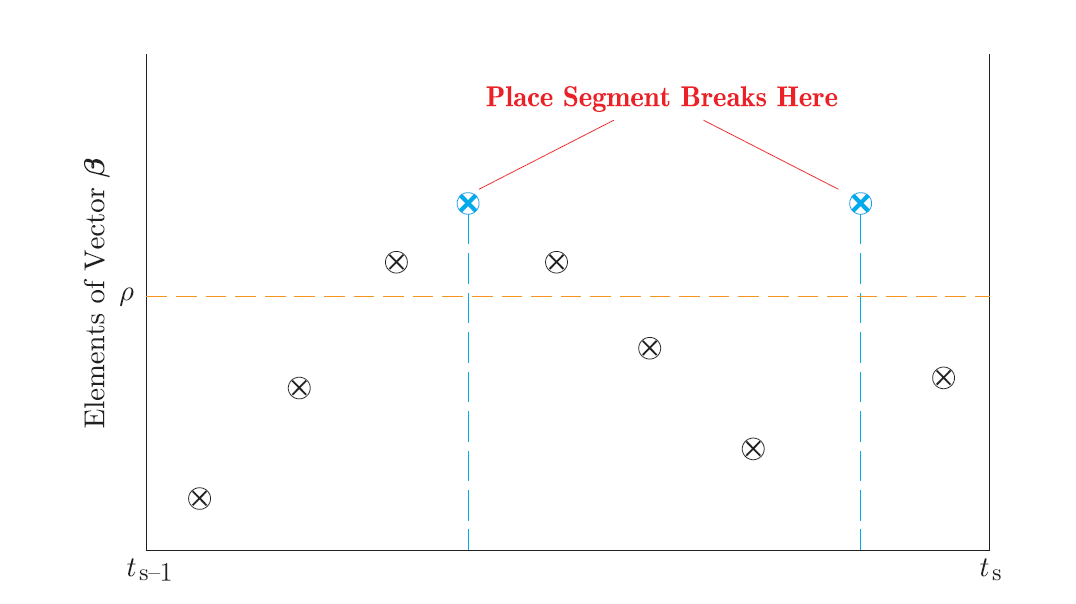
\includegraphics[width=0.8\textwidth]{figures/hp-sketch}
		\end{center}
		\caption{hp网格细化示意图}
		\label{fig:hp-sketch}
	\end{small}
\end{figure}
更多可技术细节参考\upcite{Patterson-2014-GPOPSIIMATLAB}。

\section{伪谱法快速可达域计算与分析}

可达域的计算目的是得到飞船在固定初始状态下,获得其机动包络能力。
\subsection{可达域求解策略}
求解再入可达域问题可以表示为求解不同纵程条件下的最大横程问题。即包含两步:
\begin{compactenum}
	\item 求解纵程优化问题,获得纵程的范围;
	\item 在给定纵程下,求解横程优化问题。
\end{compactenum}

首先定义纵程与横程的


\subsection{纵向航程范围获取}
最大最小纵程的轨迹设计

\subsection{可达域方法的计算结果}
程序测试通过,做出类似这样的图的效果
\begin{figure}[htb]
	\begin{minipage}{0.48\textwidth}
		\centering
		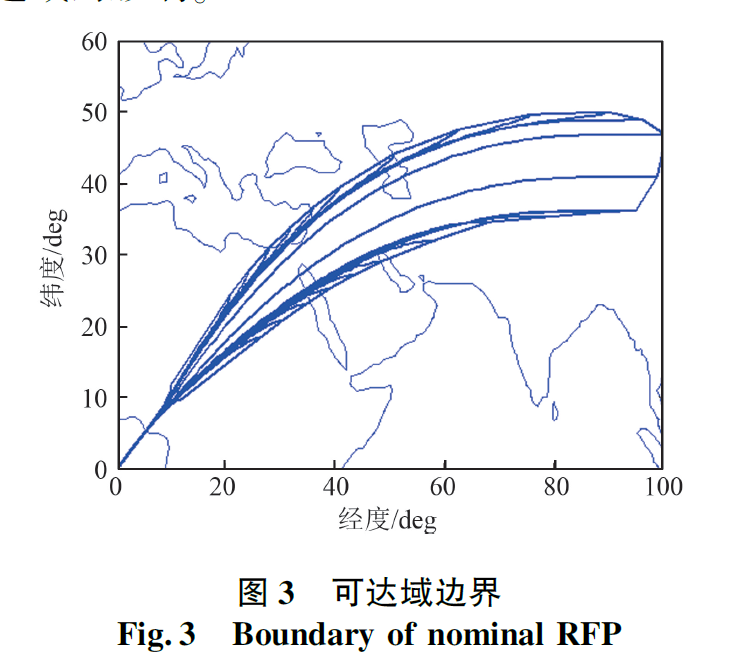
\includegraphics[width=\textwidth]{footboundary.png}
		\caption{并排第一个图}
		\label{fig:parallel1}
	\end{minipage}\hfill
	\begin{minipage}{0.48\textwidth}
		\centering
		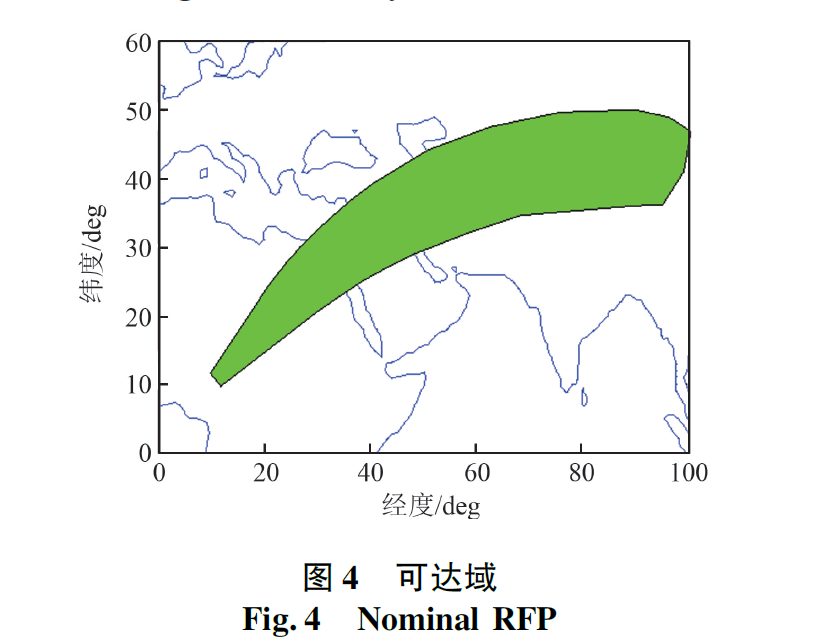
\includegraphics[width=\textwidth]{footboundary2.png}
		\caption{并排第二个图}
		\label{fig:parallel2}
	\end{minipage}
\end{figure}

\begin{figure}[htb]
	\begin{minipage}{0.48\textwidth}
		\centering
		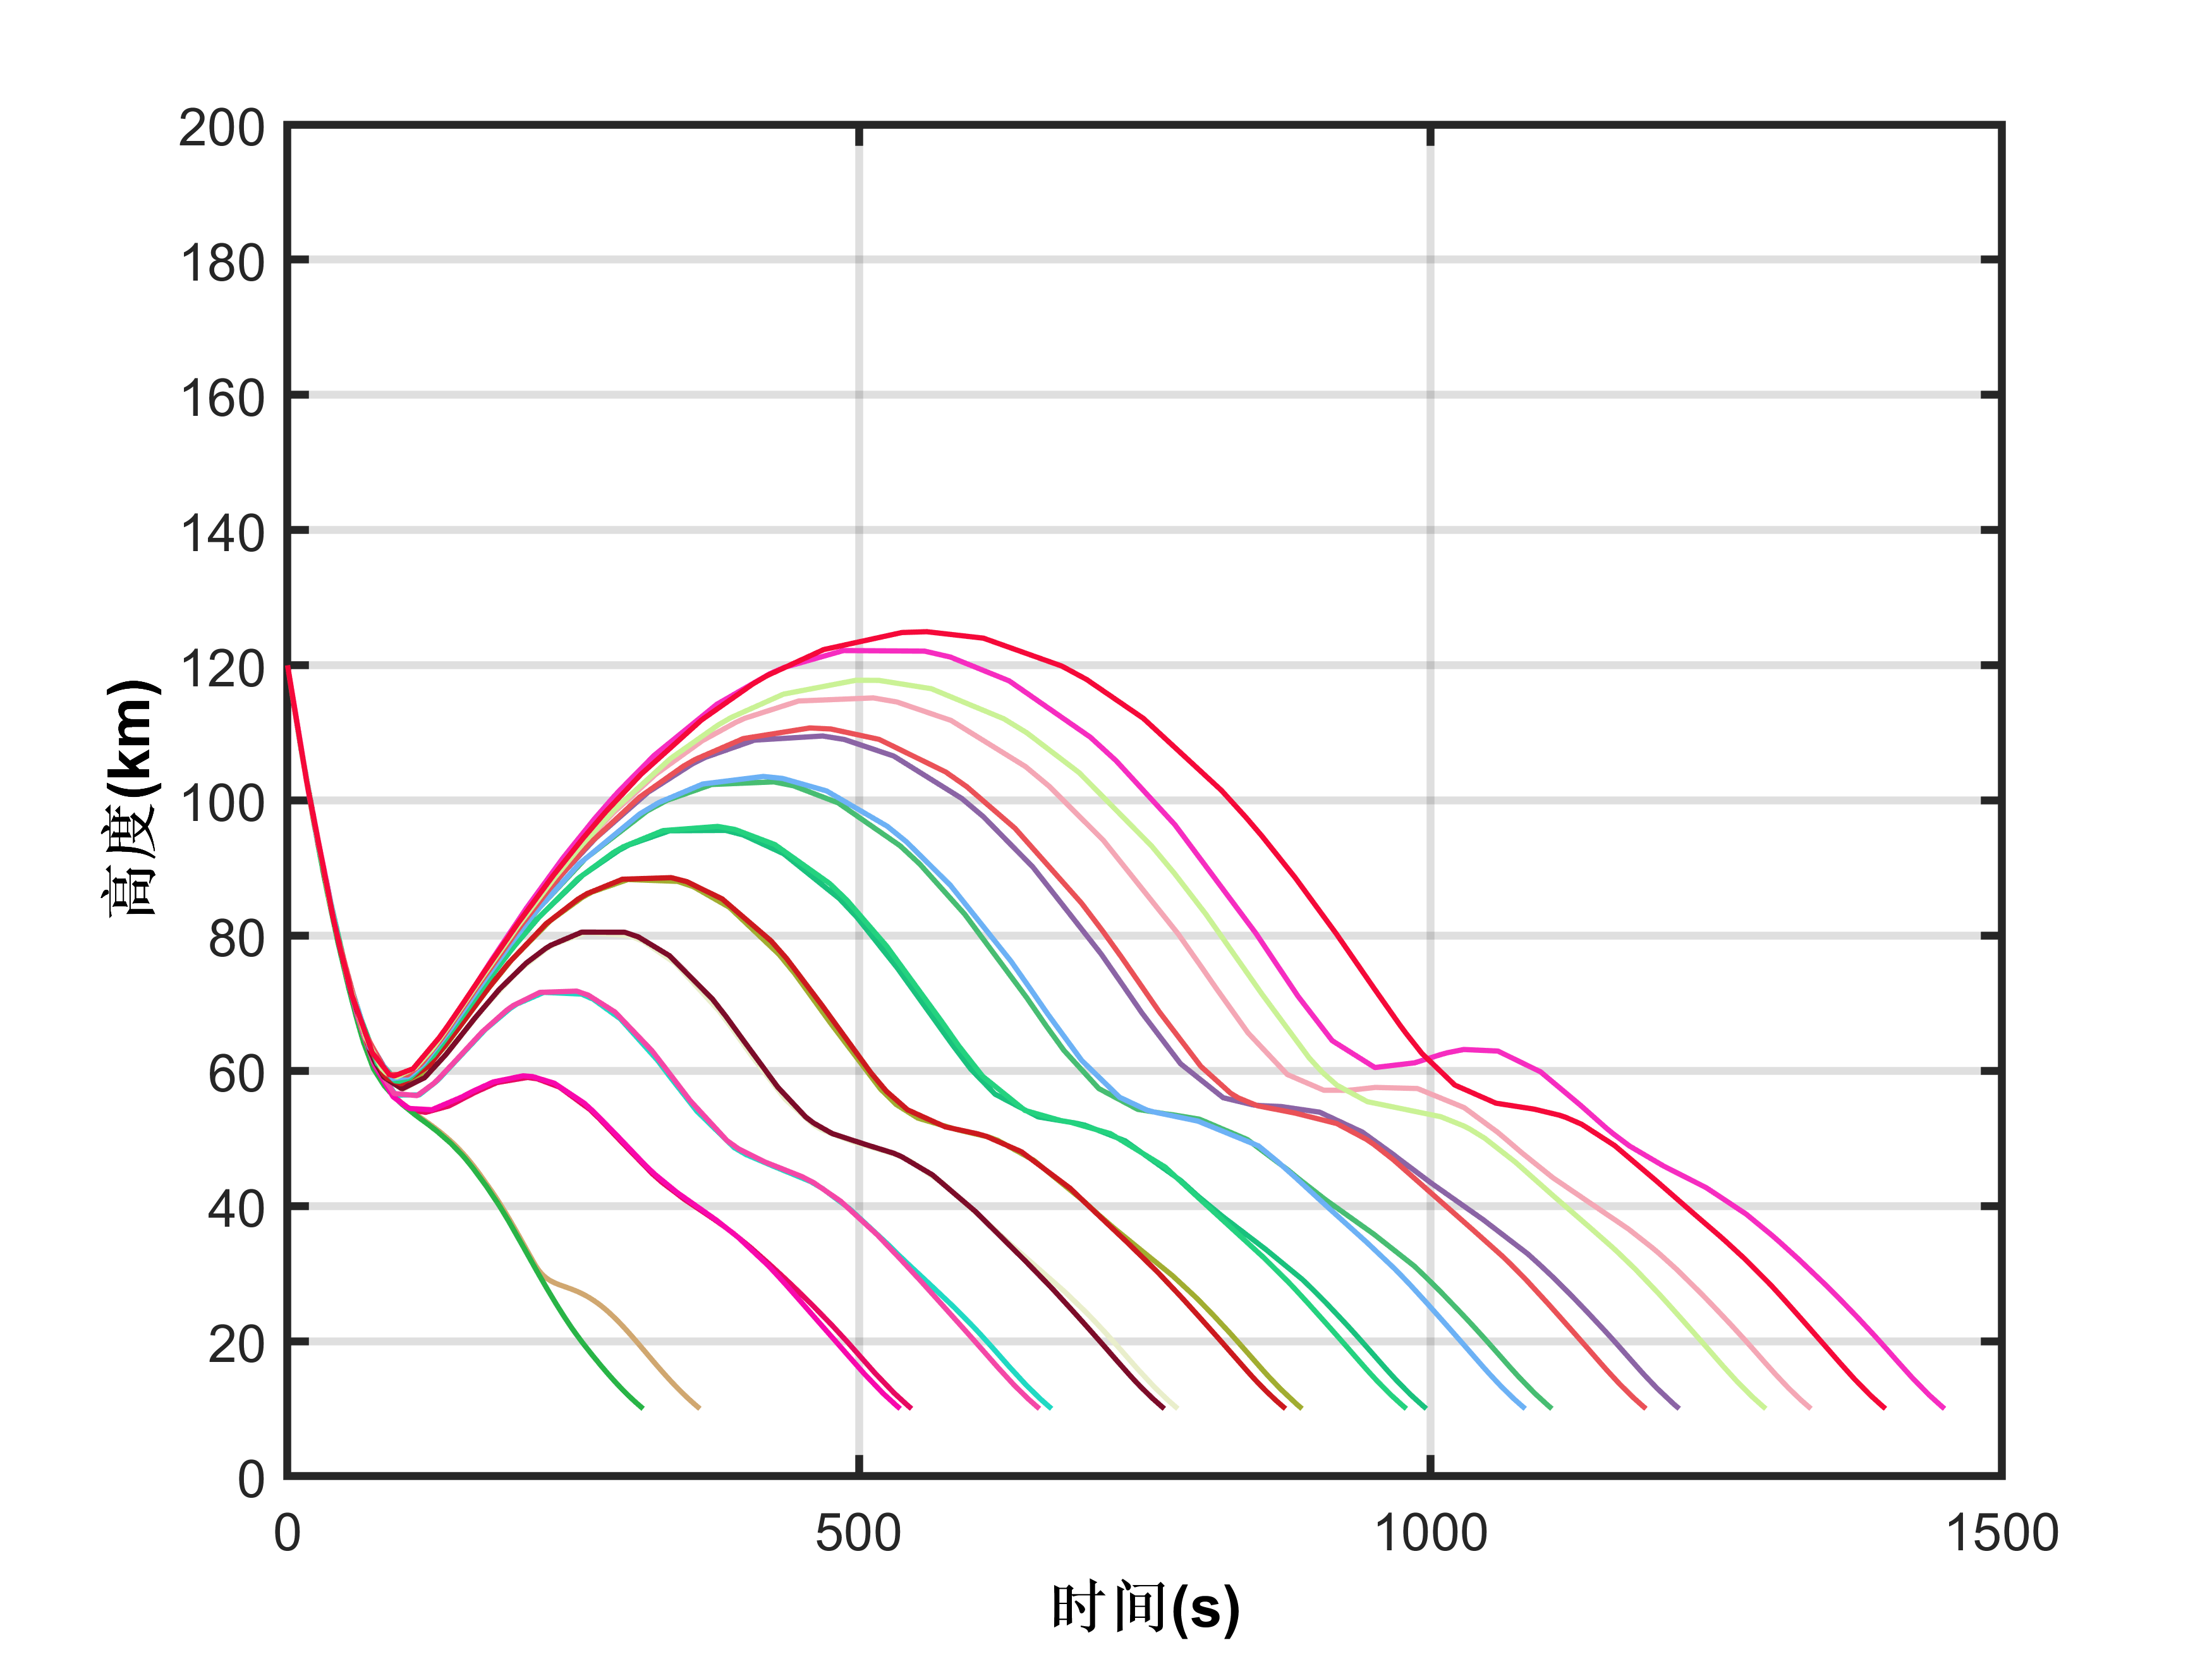
\includegraphics[width=\textwidth]{1.png}
		\caption{并排第一个图}
		\label{fig:parallel1}
	\end{minipage}\hfill
	\begin{minipage}{0.48\textwidth}
		\centering
		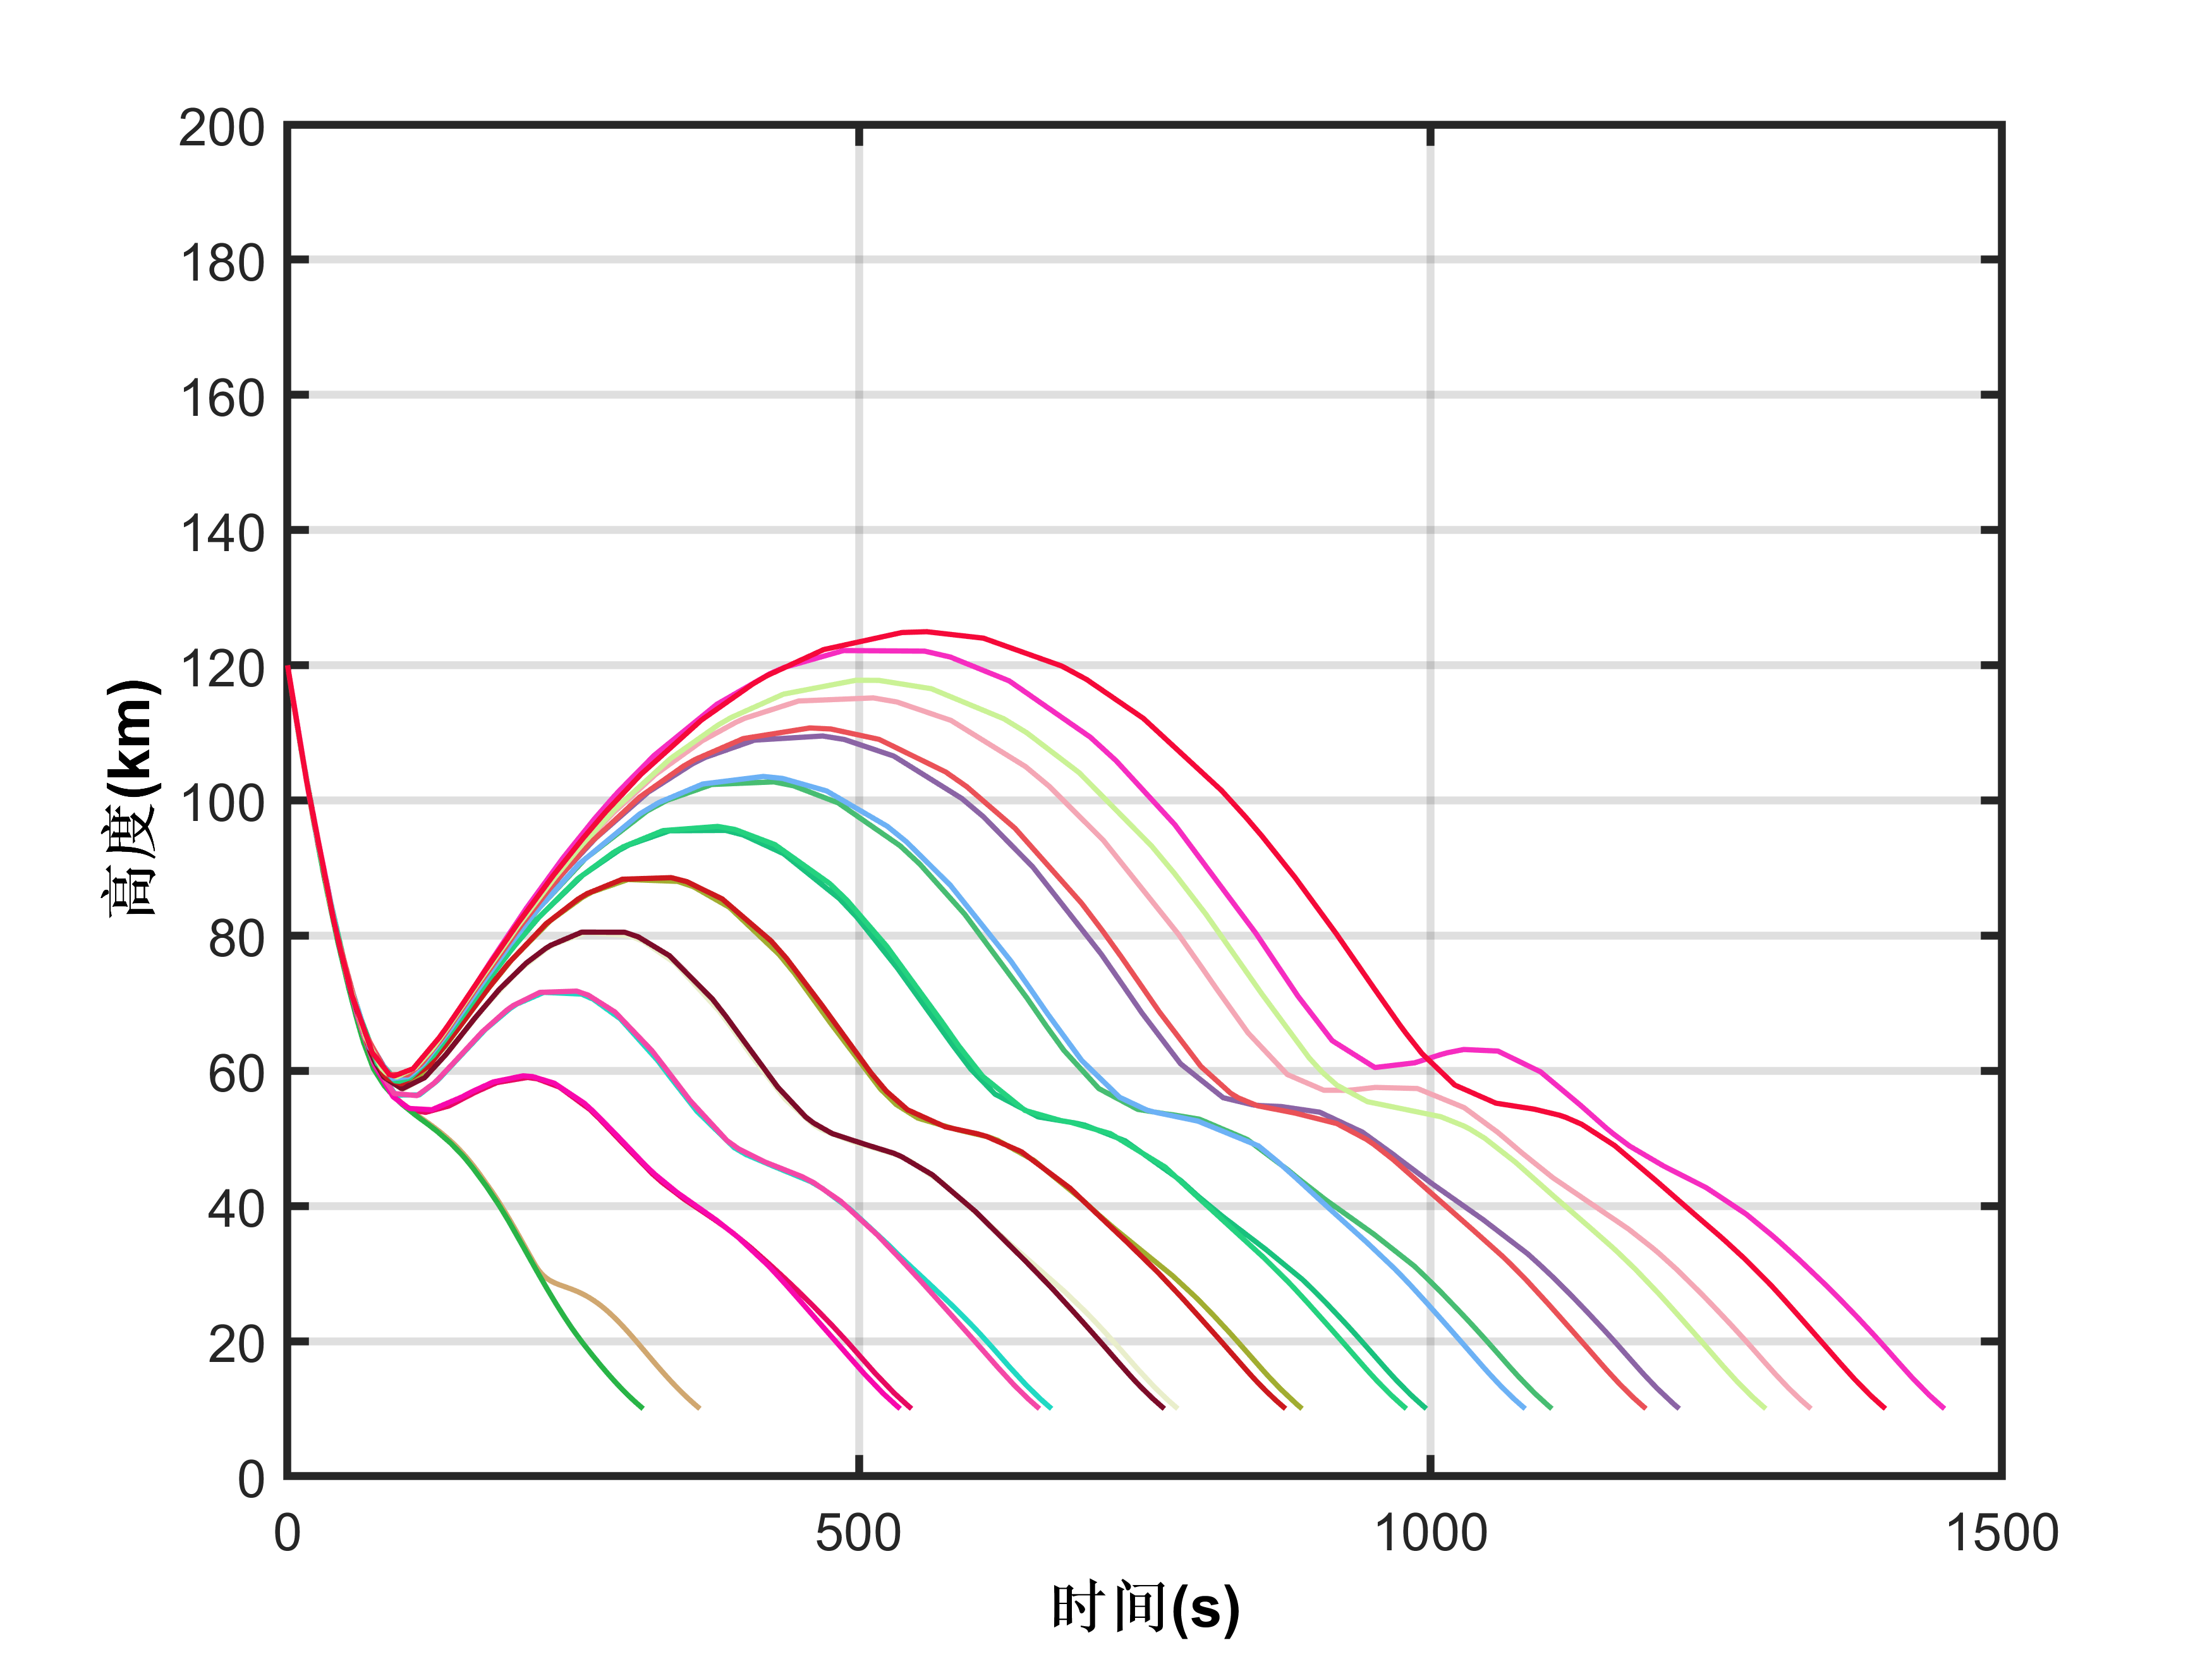
\includegraphics[width=\textwidth]{1.png}
		\caption{并排第二个图}
		\label{fig:parallel2}
	\end{minipage}
\end{figure}

\section{短航程再入轨迹设计结果对比}
\subsection{短航程再入解析轨迹设计}
短航程设计简要介绍??
\subsection{结果对比分析}
分析其中最短航程对应的参数情况,对应返回最为恶劣的情况
